%%%%%%%%%%%%%%%%%%%%%%%%%%%%%%%%%%%%
% This is the template for submission to MICRO 2022
% The cls file is modified from 'sig-alternate.cls'
%%%%%%%%%%%%%%%%%%%%%%%%%%%%%%%%%%%%

\documentclass{sig-alternate}
\usepackage{mathptmx} % This is Times font
\usepackage{listings}
\usepackage{fancyhdr}
\usepackage{xcolor}
\usepackage[normalem]{ulem}
\usepackage[hyphens]{url}
\usepackage[sort,nocompress]{cite}
\usepackage[final]{microtype}
\usepackage[keeplastbox]{flushend}
\usepackage{subfig}
\usepackage{algorithm}
%\usepackage{algorithmic}
\usepackage{algpseudocode}
% Always include hyperref last
\usepackage[bookmarks=true,breaklinks=true,letterpaper=true,colorlinks,citecolor=blue,linkcolor=blue,urlcolor=blue]{hyperref}


\newcommand{\CommentOut}[1]{}
\newcommand\TODO[1]{\textcolor{red}{TODO #1}}
\newcommand\COMMENT[1]{\textcolor{green}{COMMENT #1}}
\newcommand{\Treebeard}{{\sc {Treebeard}}}
\newcommand{\op}[1]{{\texttt {#1}}}
\DeclareMathOperator{\Tree}{\ensuremath{\tau}}

\definecolor{codegreen}{rgb}{0,0.6,0}
\definecolor{codegray}{rgb}{0.5,0.5,0.5}
\definecolor{codepurple}{rgb}{0.58,0,0.82}
\definecolor{backcolour}{rgb}{0.95,0.95,0.92}

\lstdefinestyle{c++}{language=C++,
    morekeywords={ensemble, getTree, getRoot, isLeaf, isLeafTile, traverseTreeTile, getLeafValue, loadThresholds,
                  loadFeatureIndices, loadTileShape, getChildNode, parallel, InterleavedWalk, evaluateTilePredicates,
                  getChildTile, WalkDecisionTree},    
    backgroundcolor=\color{backcolour},   
    commentstyle=\color{codegreen},
    keywordstyle=\color{blue},
    numberstyle=\tiny\color{codegray},
    stringstyle=\color{codepurple},
    basicstyle=\scriptsize,
    breakatwhitespace=false,         
    breaklines=true,                 
    captionpos=b,                    
    keepspaces=true,                 
    numbers=left,                    
    numbersep=5pt,                  
    showspaces=false,                
    showstringspaces=false,
    showtabs=false,                  
    tabsize=2
}

\lstset{style=c++}

% Ensure letter paper
\pdfpagewidth=8.5in
\pdfpageheight=11in

%%%%%%%%%%%---SETME-----%%%%%%%%%%%%%
\newcommand{\microsubmissionnumber}{654}
%%%%%%%%%%%%%%%%%%%%%%%%%%%%%%%%%%%%

\fancypagestyle{firstpage}{
  \fancyhf{}
  \renewcommand{\headrulewidth}{0pt}
  \fancyhead[C]{\vspace{10pt}\normalsize{MICRO 2022 Submission
      \textbf{\#\microsubmissionnumber} -- Confidential Draft -- Do NOT Distribute!!}\\\vspace{-25pt}} 
  \fancyfoot[C]{\thepage}
}

\pagenumbering{arabic}

%%%%%%%%%%%---SETME-----%%%%%%%%%%%%%
\title{Treebeard : An Optimizing Compiler for Tree Based ML Inference} 
%%%%%%%%%%%%%%%%%%%%%%%%%%%%%%%%%%%%

\begin{document}
\maketitle
\thispagestyle{firstpage}
\pagestyle{plain}



%%%%%% -- PAPER CONTENT STARTS-- %%%%%%%%
\begin{abstract}
  Decision tree ensembles are commonly used machine learning models
  generated by machine learning techniques like gradient boosting and random forests. 
  These models are used in a wide range of applications and are deployed at scale
  (run repeatedly on billions of data items). Several libraries such as XGBoost, 
  LightGBM, and Sklearn expose algorithms for both training and inference with 
  decision tree ensembles. While these libraries 
  incorporate a limited set of hardware-specific optimizations,
  they do not specialize the inference code to the model being used, 
  leaving significant performance on the table.

  This paper presents a compiler-based approach that automatically generates  
  efficient code for decision tree inference. 
  It develops Treebeard, an extensible compiler, which progressively lowers  
  inference code to LLVM IR through multiple intermediate abstractions.
  By applying model-specific optimizations at the higher levels, loop
  optimizations at the middle level, and machine-specific optimizations lower down,
  Treebeard can specialize inference code for each model on each supported
  hardware target. To improve model inference performance, Treebeard performs several 
  novel optimizations such as tree tiling, tree walk unrolling, and tree walk interleaving.
 
  We implement Treebeard using the MLIR compiler infrastructure and
  demonstrate the utility of Treebeard by evaluating it on a diverse set of
  tree ensemble models. Experimental evaluation demonstrates that Treebeard optimizations 
  improve average latency over a batch of inputs by 2.2X over our baseline version. 
  Further, Treebeard is significantly faster than %% other frameworks like
  XGBoost and Treelite in both single-core (2.8X and 5.1X respectively) and multi-core
  (3.2X and 2.6X respectively) settings.
\end{abstract}

\section{Introduction}
% Decision trees are among the most widely used ML models. Cite Kaggle and looking glass 
Decision tree ensembles are one of the most popular classes of machine learning models \cite{KaggleSurvey,LookingGlass}.
They are generated by machine learning techniques like gradient boosting and random forests. 
The Kaggle state of data science and machine learning survey \cite{KaggleSurvey} shows that 
these are the most widely used classes of models among data scientists. An analysis of 
several machine learning pipelines that are in production use in a real large scale web company showed that 
gradient boosting machines and random forests were the two most widely used ML algorithms in the company \cite{LookingGlass}.
Not only are decision tree based models widely used, they are also used in a diverse range of 
applications\cite{DecisionTreesOverview}. GBM models were used in the CERN large hadron collider
to classify particles based on the data collected from the collider\cite{LHCModel}. Other applications 
include search engines\cite{YahooSearch}, prediction of the financial performance of companies\cite{Finance},
medical diagnostics\cite{Med1, Med2} and recommendation and notification systems\cite{Facebook}.

% Decision tree ensemble overview
To compute the prediction of a decision tree on an input row $x$\footnote{An input row is a
vector of numbers.}, a path from the root to leaf is computed.
Each node of a decision tree has a threshold value $v$ and a feature index (or column index) $i$.
At a node, if $x_i < v$, then 
the walk moves to the left child. If not, we move to the right child. When a leaf is reached, 
the value of the leaf is returned as the prediction of the tree. 
Most decision tree based techniques combine several trees into a forest (or ensemble) to improve prediction accuracy.
To compute the prediction of the forest, the prediction of each tree is computed and these predictions are 
then combined (usually by adding them). 

% Inference on decision trees is hard 
% Pointer chasing -- cache performance, branch prediction, dependency stalls, not easy to vectorize
Given the wide spread use of decision tree ensembles, the ability to perform high throughput and low latency inference is important.
\TODO{AP Since we don't talk about latency or throughput explicitly, should we be saying this?}
However, optimizing the tree walks required for decision tree inference on modern CPUs is not straight-forward. 
Firstly, naively implemented tree walks have poor spatial and temporal locality and therefore poor cache performance \cite{FAST,MilindTreeVectorization}.
Additionally, since the decision of which node to evaluate next can only be made after evaluating the current node,
true dependencies between instructions cause several pipeline stalls. Also, using SIMD instructions to accelerate 
tree walks is extremely challenging \cite{MilindTreeVectorization}.

Several systems like XGBoost\cite{XGBoost}, LightGBM\cite{LightGBM} and Sklearn\cite{Sklearn} implement
decision tree ensemble inference. These are libraries and implement some optimizations. However, these optimizations are hand
coded and need to be manually rewritten or redesigned for every target that is supported. Also, these 
systems cannot apply specialize inference code depending on the model. A compiler based approach is 
needed to address these problems. However, existing compilers only support fixed code generation techniques\cite{Treelite, Hummingbird}.
To fill the need for an extensible compiler infrastructure for decision forest ensembles, we design and 
build \Treebeard{}\footnote{In J. R. R. Tolkein's The Lord of the Rings, Treebeard was the oldest of the Ents left in Middle-earth, an 
ancient tree-like being who was a ``shepherd of trees''.}, an optimizing compiler for decision tree ensemble inference.
Our motivations for building \Treebeard{} are as follows. 
\begin{enumerate}
  \item Existing libraries \cite{XGBoost, Treelite, LightGBM, VPred} perform specific optimizations and are hard to maintain as hardware evolves. 
  Additionally, they cannot tailor inference code to the specific model being used. Past work has identified that the optimizations required change with the model
  and architectural parameters like cache size\cite{CacheConscious1, CacheConscious2, VPred}. 
  \item The repeated effort to optimize and maintain libraries on several targets is prohibitive. The proliferation of new architectures
  further exacerbates this problem. Compilers have been successful in alleviating this problem in other domains\cite{Halide, TVM}.
  However, no such compiler infrastructure currently exists for decision tree ensembles.
  \item Currently, no system exists that allows a thorough exploration of the optimization space for decision tree ensemble inference. 
  Compilers have been successful in addressing this problem with ML models like DNNs \cite{TVM, Tiramisu, XLA}. However, compiler techniques for
  decision tree ensembles are less well studied.
\end{enumerate}

We make the following contributions.
\begin{enumerate}
  \item We design and build \Treebeard{}, an extensible compiler infrastructure for decision tree model inference. The 
  infrastructure is built to allow exploration of optimization and code generation techniques. \TODO{Is this claim too grand?}
  \item We develop a general infrastructure for the vectorization of decision tree walks based on grouping tree nodes into ``tiles''.
   This includes general support for code generation and the in-memory representation of tiled trees. The infrastructure can be 
   used to tile trees based on different cost functions.
  \item We show that trees can be tiled using different cost functions. We present two novel tiling methods that are implemented
  using the general tiling infrastructure. 
  \item We design and implement various model and loop transformations that significantly improve generated inference code performance 
  to show the power of the proposed framework.
\end{enumerate}



\section{Treebeard Overview}
Figure \ref{Fig:CompilerStructure} shows the high level structure of \Treebeard{}. 
The input to \Treebeard{} is a serialized decision tree ensemble. 
%% Popular frameworks like XGBoost and LightGBM are supported and the system is easily extensible to other frameworks.
Given an input model our compiler generates optimized inference code. Specifically it generates a 
callable batch inference function \texttt{predictForest} that, given an array of input rows, computes an
array of model predictions. 
 
\Treebeard{} specializes the code generated for inference by progressively optimizing and lowering a 
high level representation of the \texttt{predictForest} function down to LLVM IR \cite{LLVM}.
%% By \textbf{\emph{lowering}}, we mean 
\textbf{\emph{Lowering}} is the process of transforming an operation at a higher 
abstraction to a sequence of operations at a lower abstraction. Optimizations in \Treebeard{} 
are implemented using a combination of annotation and lowering. An operation at a higher 
abstraction is annotated with attributes that indicate what kind of optimization is 
to be performed while lowering it. The lowering transformation uses this information to generate 
optimized lower level code. For example, tree tiling and loop ordering (figure \ref{Fig:Overview} 
shows two possible loop orders -- one tree at a time and one row at a time) are decided 
at the highest abstraction. These decisions are communicated to the lowering pass 
which explicitly encodes them in the lowered IR as shown in Figure \ref{Fig:Overview}.

%Treebeard first constructs a high level representation of the decision forest inference operation.
\Treebeard{}'s IR has three abstraction levels as shown in Figure \ref{Fig:Overview}.  
At the highest level (HIR), the input model is represented as a collection of binary trees. This is shown 
in the second row of Figure \ref{Fig:Overview}. At this level of abstraction,
\Treebeard{} tiles nodes together to transform a binary tree into an $n$-ary tree 
and decides what order trees are to be traversed in. In the example in the figure, 
trees are tiled with a tile size of 2. Tiling is indicated using colored elipses drawn 
around nodes that are in the same tile. Tree reordering is another transformation that is performed at this abstraction. 
One objective of tree reordering is to group identically structured trees so that they can share the same traversal code
to improve locality in the instruction cache.  Alternative objectives for reordering can easily be supported.
With the tiling shown in Figure \ref{Fig:Overview}, Tree1 and Tree3 have depth 1, while Tree2 has a depth of 2.
Therefore, the trees are reordered so that Tree1 and Tree3 are together. 

The high level IR is then lowered to a mid-level IR (MIR). The aim of MIR is 
to allow optimizations that are independent of the final memory layout of the model. 
The lowering to MIR performs loop transformations like loop tiling, permutation, parallelization and unrolling.
At this level of the IR (the third row in Figure \ref{Fig:Overview}),
the order in which trees, input row pairs are walked is explicitly represented in the IR using loop nests.
Figure \ref{Fig:Overview} shows two possible ways that loop nests could be generated -- the first
walks all rows for one tree before moving to the next tree while the second walks all trees for 
one row before moving to the next row. Another aspect handled by this lowering is the fissing of 
loops to make sure that trees with the same structure share code. Here, both versions of MIR shown 
ensure that Tree1 and Tree3 share the same traversal code, while traversal code for Tree2 is different.
Additionally, tree walk optimizations, such as tree walk unrolling (shown in figure \ref{Fig:Overview}) and 
peeling are performed on the MIR.

\Treebeard{} then further lowers the IR to explicitly represent the memory layout of the model. Buffers to hold model 
values are inserted into the generated code and all tree operations in the mid-level IR are lowered to explicitly 
reference these buffers. Additionally, at this level of the IR, \Treebeard{} generates vectorized code to take 
advantage of SIMD instructions where applicable. Finally, the inference function is translated to LLVM IR and 
JIT compiled to executable code. 

%The following sections describe each level of the IR and their lowering in more detail.

\begin{figure}
  \centering
  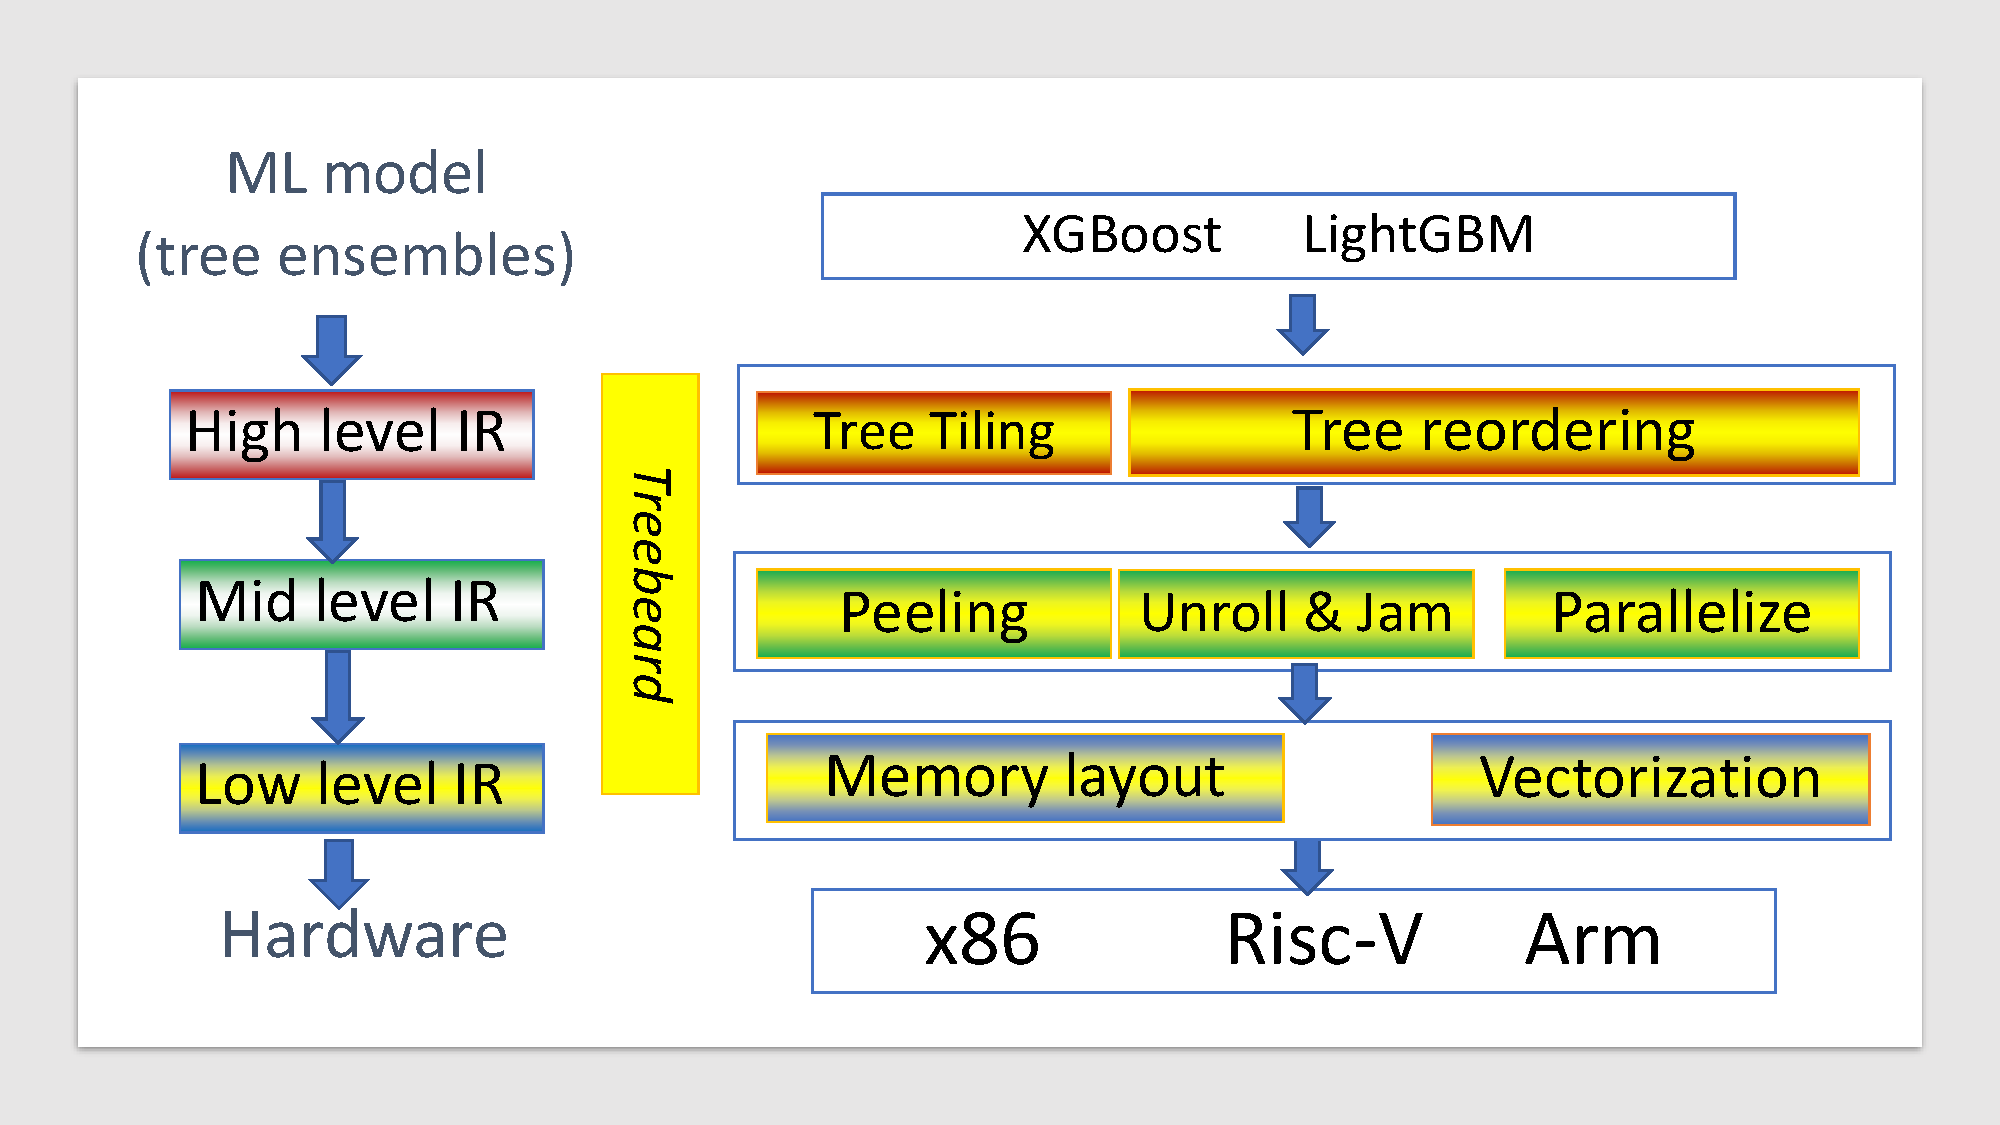
\includegraphics[width=\linewidth]{figures/compiler.pdf}
  \caption{Treebeard compiler structure}
  \label{Fig:CompilerStructure}
\end{figure}

\begin{figure*}
  \centering
  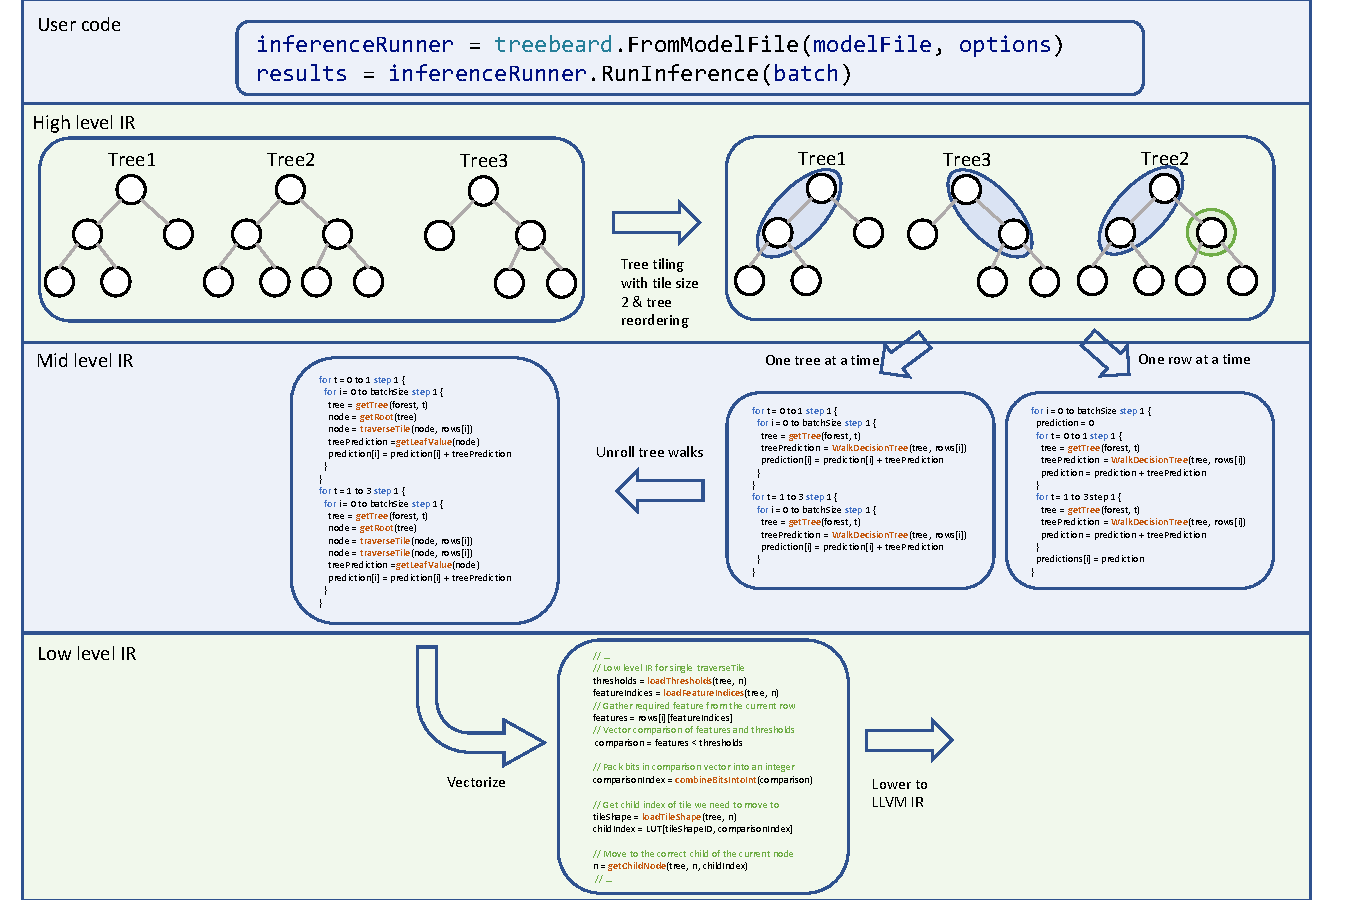
\includegraphics[width=\textwidth]{figures/OverviewExample.pdf}
  \caption{\Treebeard{} IR lowering and optimization details. The three abstraction levels in Treebeard's IR are shown. The
           high level IR is a tree based IR to perform model level optimization, the mid-level IR is for
           loop optimizations that are independent of memory layout and the low level IR allows us to perform
           vectorization and other memory layout dependent optimizations.}
  \label{Fig:Overview}
\end{figure*}



%\TODO{Should we describe the dialect's type system?}
% \TODO{Kr : consider focusing on the example instead of verbose description of optimizations. This section can be short, descriptions can come in later sections.}
% \subsection{High Level IR}
% As a first step Treebeard parses the input and generates a single MLIR operation, \texttt{predictForest} that represents inference using the input model on a set of rows. 
% At this level the operator simply contains a collection of binary trees. Two optimizations, tiling and tree ordering are applied at this level. The objective of tiling is to group nodes together so that the tree can be walked one tile at a time instead of one node at a time. We demonstrate that tiling can specialize the traversal of individual trees to either balance heavily skewed trees or proritize walks leading to higher probability leafs. Figure~\ref{ttile} shows examples of the tiling transformation. \TODO{kr: draw and explain example}. The objective of tree reordering is to group identically structured trees so that they can share the same traversal code. The predictForest function is now lowered to MIR with separate loop nests generated for traversing groups of identical trees. The generated MIR code is as shown below. 
% \TODO{show unoptimized loop nest as a listing}.

%The operation contains within it a tree based representation of the model that can be manipulated by optimizing transformations. Transformations on the model such as tiling, tree reordering and leaf padding are done at this level. The structure of the loop nest to walk the iteration space of trees and inputs is also decided at this level of the IR. \TODO{Should we mention that there is a scheduling language to decide this?}
% \begin{lstlisting}[language=C++]
% func Predict(float rows[batchSize]) {
%   predictions = predictForest(rows) 
%   return rows
% }
% \end{lstlisting}

% \subsection{Mid Level IR}
% The Mid Level IR optimizes the loop structures and tree walks. Firstly, the order in which the iteration space of trees and inputs is walked is determined and by re-ordering the loop nesting if necessary. Also, operations such as \texttt{isLeaf}, \texttt{traverseTile}, \texttt{getLeafValue} are introduced so that the traversal of trees explicitly represented. The following listing shows the IR for inference using a model with four trees on an input batch with two rows. The listed IR walks all trees for one input row before moving to the next row. One important point to note here is that details such as the data structure used for the trees are not explicitly encoded in the IR. This allows us to reuse optimization and lowering passes on this level of the IR regardless of what the final in memory representation of the model is.

% \begin{lstlisting}[style=c++]
%   // Constant that represents the model being compiled
%   forest = ensemble(...)
%   for i = 0 to 2 step 1 {
%     prediction = 0
%     for t = 0 to 4 step 1 {
%       tree = getTree(forest, t) 
%       node = getRoot(tree)
%       while (isLeaf(tree, n)==false)  do {
%         node = traverseTreeTile(tree, node, rows[i])
%       }
%       treePrediction = getLeafValue(tree, node)
%       prediction = prediction + treePrediction
%     }
%     predictions[i] = prediction
%   }
% \end{lstlisting}

% The IR listed above is a simplification of the actual IR. The actual IR is strongly typed and in SSA form.

% \subsection{Low Level IR}
% The IR is finally lowered to a form where the in memory representation of the model is made explicit. Buffers to hold the model values are inserted into the generated code and all tree operations in the mid-level IR are lowered to explicitly reference these buffers. The semantics of all operations are made explicit. For example, \texttt{traverseTreeTile} is lowered into a series of operations to load thresholds, feature indices and features, compare the features with the thresholds and compute the next node to evaluate. This IR is then lowered directly to LLVM IR and JITted.


%\section{Optimizations}
\section{high level IR Optimizations}
This section describes tiling and tree ordering, two optimizations performed at the highest level of abstraction. Recall that at this level the \op{predictForest} operator is abstractly represented by just a set of trees. 

%\TODO{This section needs a better name!}
\subsection{Notation}
\TODO{Notation needs to be introduced in the background section}
We represent a decision tree by $T = (V, E, r)$ where $V$ is the set of nodes, $E$ the set of edges and
$r \in V$ is the root. For each node $n \in V$, the following are given.
\begin{enumerate}
    \item $threshold(n) \in \mathbb{R}$ which gives the threshold value for $n$.
    \item $featureIndex(n) \in \mathbb{N}$ which gives the feature index for $n$.
    \item $left(n) \in V$, the left child of $n$ or $\emptyset$ if $n$ is a leaf. If $left(n) \neq \emptyset$, then $(n, left(n)) \in E$.
    \item $right(n) \in V$, the right child of $n$ or $\emptyset$ if $n$ is a leaf. If $right(n) \neq \emptyset$, then $(n, right(n)) \in E$.
\end{enumerate}
We use $L \subset V$ to denote the set of leaves. 

\subsection{Tiling}

Treebeard vectorizes tree walks by grouping nodes of a decision tree into \textbf{\emph{tiles}}. The nodes in a tile are evaluated concurrently using vector instructions. Once the nodes of the current tile are evaluated, a look up table is used to compute which child of the current tile to move to next. The listing below shows at a high level how a tiled tree is walked. 
\begin{lstlisting}[style=c++]
  // A lookup table that determines the child index of
  // the next tile given the tile shape and the outcome
  // of the vector comparison on the current tile
  int16_t LUT[NUM_TILE_SHAPES, pow(2, TileSize)]
  
  ResultType Prediction_Function(...) {
    // ...
    Node n = getRoot(tree)
    while (isLeaf(tree, n)==false) do {
      thresholds = loadThresholds(tree, n)
      featureIndices = loadFeatureIndices(tree, n)
      // Gather required feature from the current row
      features = rows[i][featureIndices]
      // Vector comparison of features and thresholds
      comparison = features < thresholds
      
      // Pack bits in comparison vector into an integer
      comparisonIndex = combineBitsIntoInt(comparison)
      
      // Get child index of tile we need to move to
      tileShape = loadTileShape(tree, n)
      childIndex = LUT[tileShapeID, comparisonIndex]
      
      // Move to the correct child of the current node
      n = getChildNode(tree, n, childIndex) 
    }
    ThresholdType prediction = getLeafValue(n)
    // ...
  }  
\end{lstlisting}

To evaluate the current tile, the vector of thresholds is first loaded (\texttt{loadThresholds}). This vector contains the thresholds of all nodes in the tile. Then, the features required for comparison are gathered into a vector (lines 11 and 13). The feature vector is compared to the threshold vector and the child tile to move to is determined (lines 15 to 25). More details about tile shapes and the look up table are presented in subsequent sections.

\subsection{Tiles and Tile Shapes}
A \textbf{\emph{tile}} is a collection of connected non-leaf nodes of a decision tree. The path connecting any pair of nodes in the tile must fully be contained within the tile. The tile size $n_t$ is the number of nodes contained in a tile.

Informally, the \textbf{\emph{tile shape}} is the shape of the region that encloses all nodes in a tile in a diagram of the decision tree. More formally, for a tile size $n_t$, each unique legal binary tree containing $n_t$ nodes (nodes being indistinguishable) corresponds to a tile shape.

Figure \ref{Fig:TileSize3Shapes} enumerates all tile shapes with a tile size of 3. There are a total of 5 tile shapes with size 3. The number of tile shapes with a tile size $n_t$, denoted by $NTS(n_t)$ is given by the following equation. 

\begin{equation}
  NTS(n) = \sum_{k=0}^{n-1} NTS(k) \times NTS(n-k-1)
\end{equation}

where $NTS(0) = NTS(1) = 1$.

\begin{figure}
  \centering
  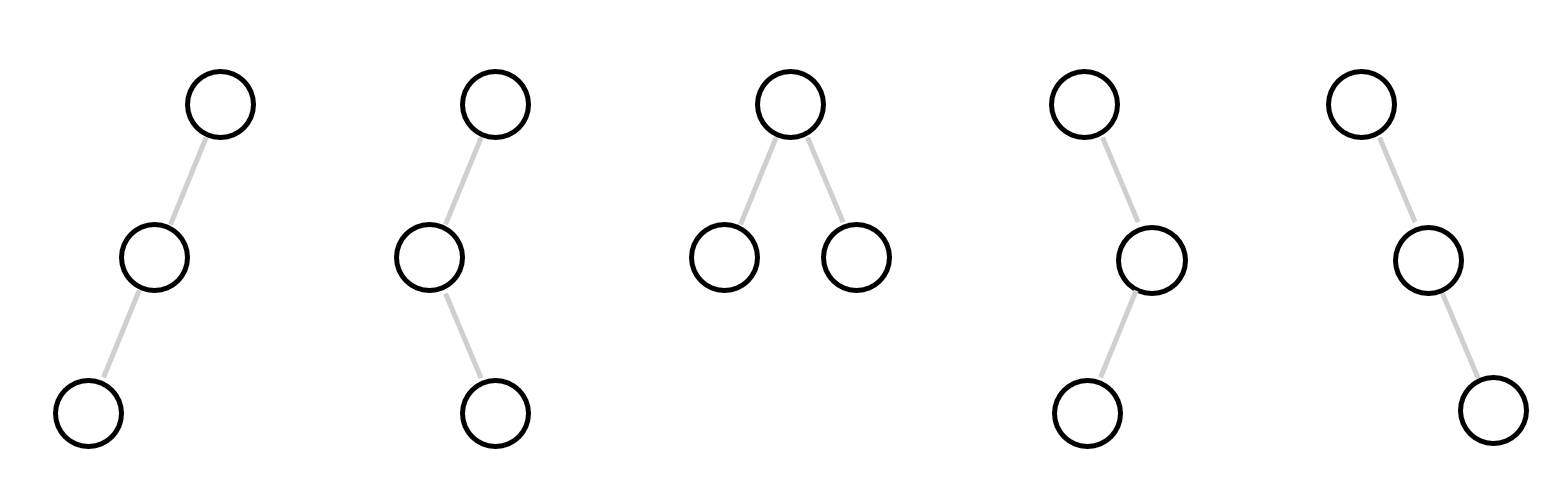
\includegraphics[width=\linewidth]{figures/TileShapes_Size3.PNG}
  \caption{All possible tile shapes with a tile size $n_t=3$}
  \label{Fig:TileSize3Shapes}
\end{figure}

\subsection{Valid Tiling of a Tree}
A tiling $\mathcal{T}$ of the tree $T = (V, E, r)$ with tile size $n_t$ is a partition $\{ T_1, T_2, ... ,T_m \}$ of the set $V$ such that 
\begin{enumerate}
    \item $T_1 \cup T_2 ... \cup T_m = V$
    \item $T_i \cap T_j = \emptyset$ for all $i, j \in [1, m]$ and $i \neq j$
    \item $|T_i| \leq n_t$ for all $i \in [1, m]$
    \item $\forall l \in L$ : $l \in T_i \rightarrow v \notin T_i \;\; \forall v \in V \backslash \{l\}$
    \item Tiles are \textbf{maximal}, i.e. if $|T_i| < n_t$, then there is no $v \in V\backslash \{ T_i \cup L \}$ such that $(u, v) \in E$ for some $u \in T_i$. 
    \item Tiles are \textbf{connected}, i.e. for an $u, v \in T_i$, there is a (undirected) path connecting $u$ and $v$ fully contained in $T_i$.
\end{enumerate} 

\TODO{AP We need to talk about how tiling is specified in the compiler}

\subsection{Tiled Trees}
A tiling transformation communicates the tiling to the Treebeard infrastructure by assigning a tile ID to each node in the decision tree. Using these tile IDs, Treebeard checks the validity of the tiling and then contructs a tree whose nodes are tiles. We call this tree the \textbf{\emph{tree of tiles}}. \TODO{We need a better name for this}
Figure \ref{Fig:ValidTilingTileSize3} shows a valid tiling with tile size 3 and the tree of tiles constructed by Treebeard. Three nodes are grouped into each of the tiles $t_1$ and $t_2$ as shown. Each tile is collapsed into a single node in the tree of tiles. However, each leaf in the original tree becomes a leaf in the tree of tiles.

\begin{figure}
  \centering
  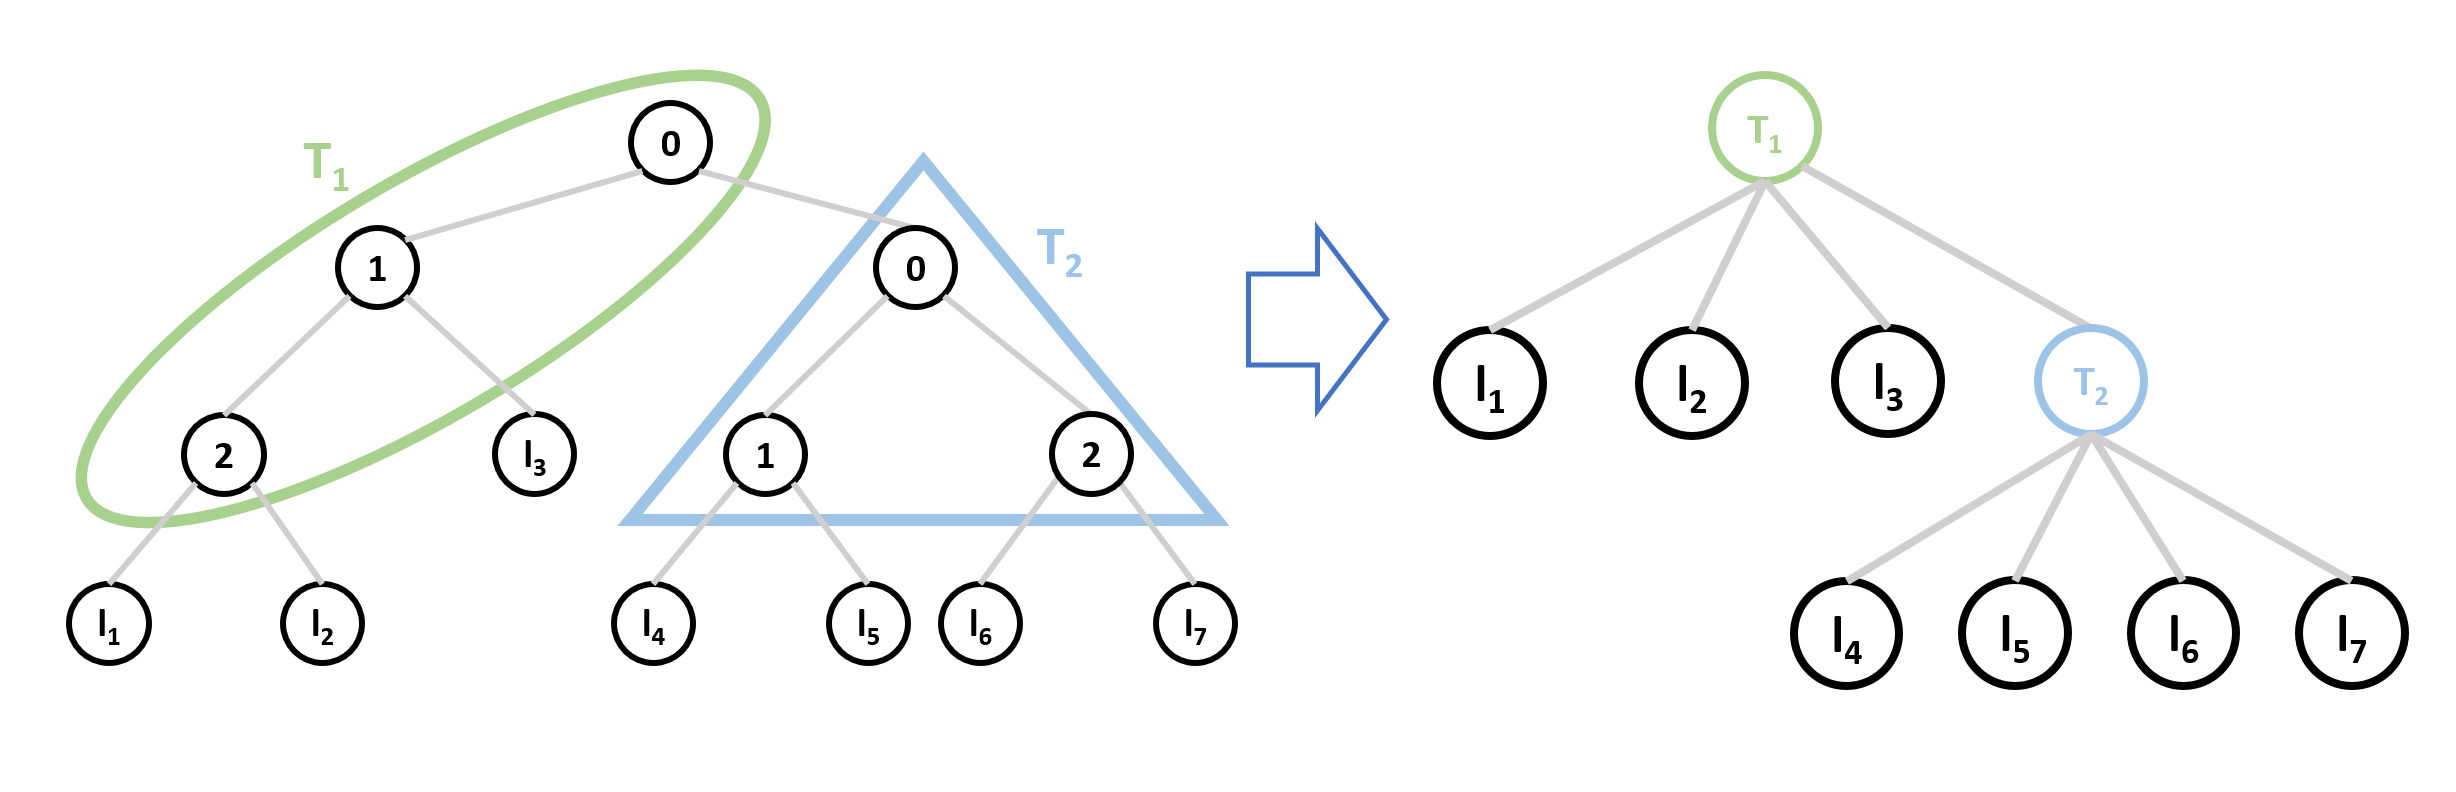
\includegraphics[width=\linewidth]{figures/TiledTree_Size3.PNG}
  \caption{Example of a valid tree tiling with a tile size $n_t=3$}
  \label{Fig:ValidTilingTileSize3}
\end{figure}

Treebeard maintains the following invariants.
\begin{enumerate}
  \item All tiles in a tree are the same size $n_t$. If the tiling produces any smaller tiles, these are padded by inserting dummy nodes to make them the required size.
  \item Nodes within tiles are always ordered in level order and left to right within a level. The numbering of the nodes in the above diagram shows this node order.
  \item Children of a node are numbered from left to right (regardless of level). For example, $l_1$ is the first child of $t_1$, $l_2$ is the second and so on.
\end{enumerate}
    
\subsection{Tile Shapes and Decision Tree Inference}
\label{Sec:TileShapesAndDecisionTreeInference}
Treebeard uses vector instructions to accelerate decision tree walks. Vector instructions are used to evaluate the predicates of all the nodes in a tile simultaneously. However, once the predicates of all the nodes in the tile are evaluated, computing the next tile to move to, given the outcome of the comparison depends on the tile shape of the current tile. To illustrate this problem, consider the case of the tiles of size 3 shown in figure \ref{Fig:TileTraversalTileSize3}. 
\begin{figure}
  \centering
  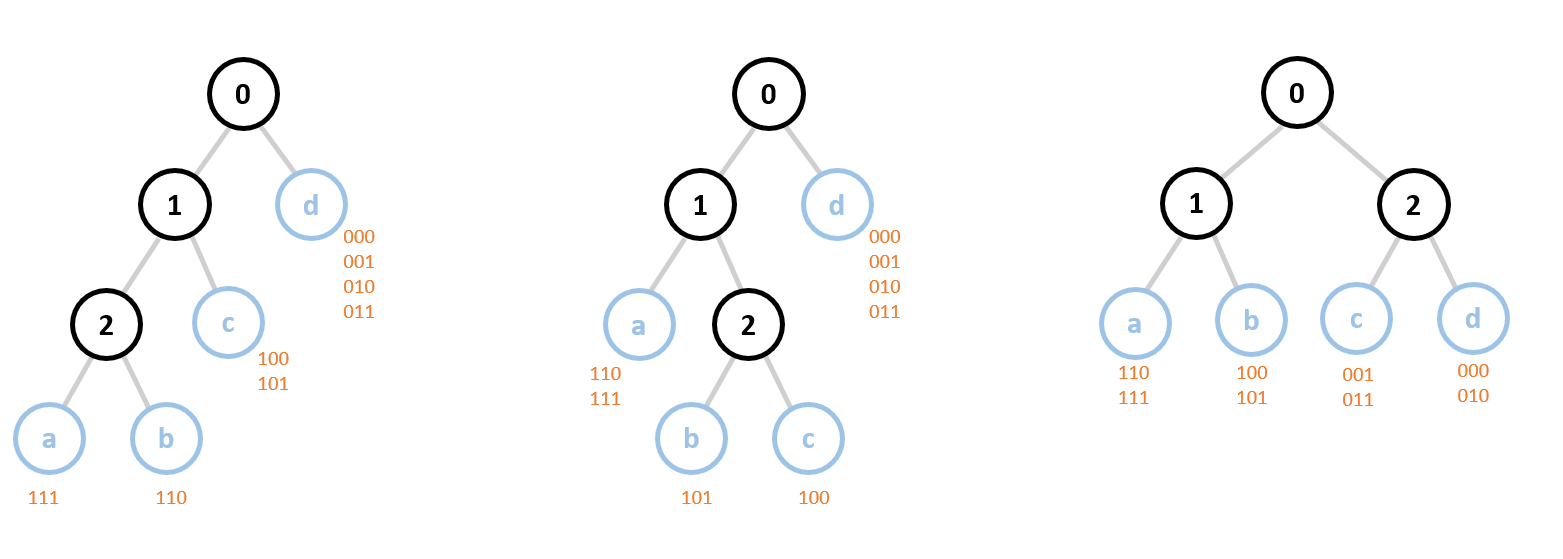
\includegraphics[width=\linewidth]{figures/TileTraversal_Size3.PNG}
  \caption{Example tile traversals with tile size $n_t=3$}
  \label{Fig:TileTraversalTileSize3}
\end{figure}
The diagram shows 3 of the 5 possible tile shapes for a tile size of 3. The nodes drawn in black are members of the tile $t_1$. The nodes in blue are the entry nodes of the children tiles of $t_1$. \TODO{Define entry nodes}

To traverse a tile on an input row, first, the predicate of each node in the tile is computed. Subsequently, we need to determine which of the child tiles to move to next. Note that a true predicte (bit value 1) on a node implies a move to the left child and a false predicate (bit value 0) implies a move to the right child.

In the diagram, the bit strings (written in red) show which child we need to move to given the outcomes of the comparison (the bits represent the comparison outcomes of nodes and are in the order of the nodes in the tile -- marked 0, 1 and 2 in the diagram, i.e., the MSB is the predicate outcome of node 0 and the LSB the predicate outcome of node 2). For example, for the first tile shape, if the predicate of all nodes are true (i.e. the comparison outcome is 111), the next node to evaluate is $a$. However, if the predicate of node 1 is false, then we need to move to $d$ regardless of the outcomes of nodes 2 and 3. It is easy to see from the diagram that, depending on the tile shape, the same predicate outcomes can mean moving to different children. For example, for the outcome "011", the next tile is the 4th child (node $d$) for the first two tile shapes while it is the 3rd child for the other tile shape (node $c$).

\subsection{Lookup Table}
A lookup table (LUT) is used to solve the problem described in section \ref{Sec:TileShapesAndDecisionTreeInference}, i.e. given the outcome of the comparisons on all nodes in a tile, determine the child tile we should evaluate next. The LUT is indexed by the tile shape and the comparison outcome. Formally, the LUT is a map.
\[
LUT : (TileShape, < Boolean \times n_t >) \rightarrow [0, n_t] \subset \mathbb{N}
\]

where $n_t$ is the tile size, $< Boolean \times n_t >$ is a vector of $n_t$ booleans. The value returned by the LUT is the index of the child of the current tile that should be evaluated next. For example, if we are evaluating the first tile $t$ in figure \ref{Fig:TileTraversalTileSize3}, and the result of the comparison is 110, then $LUT(TileShape(t), 110)=1$ since the tile we need to evaluate next is the tile with node $b$, which is the second child of the current tile.

In order to realize this LUT in generated code, Treebeard associates a non-negative integer ID with every unique tile shape of the given tile size. The result of the comparison, a vector of booleans, can be interpreted as a 64-bit integer. Therefore, the LUT can be implemented as a 2 dimensional array.
\begin{lstlisting}{style=c++}
  int16_t LUT[NTS(n_t), pow(2, n_t)]  
\end{lstlisting}

Treebeard computes the values in the LUT statically as the tile size is a compile time constant.

\subsection{In Memory Representation of Tiled Trees}
Treebeard currently has two in memory representations for tiled trees - an array based representation and a sparse representation. Both representations use an array of structs to represent all tiles of the model. 

\subsubsection{Array Based Representation}
\label{sec:ArrayBased}
Each tree in the model is represented as an array of tiles using the standard representation of trees as arrays. The root node is at index 0 and for a node at index $n$ in the array, the index of its $i^{th}$ child is given by $(n_t + 1) n + (i + 1)$ (every node in the tree of tiles has $n_t + 1$ children). A tile is represented by an object of the following struct.
\begin{lstlisting}{style=c++}
  struct Tile {
    // A vector of TileSize elements
    <ThresholdType x TileSize> thresholds; 
    <FeatureIndexType x TileSize> featureIndices;
    // Integer that identifies the tile shape
    TileShapeIDType tileShapeID; 
  };  
\end{lstlisting}
\TODO{AP Is this level of detail really needed? Also, the vector type notation needs to be introduced somewhere.}
Even though this representation is simple, the memory required for reasonable sized models is very large. The memory footprint is up to 20X that of the scalar representation. This memory bloat causes a performance degradation because the span of the L1 TLB is not sufficient to efficiently translate addresses for the whole model. \TODO{AP There are also some cache misses. Write this better.} Storing leaves as full tiles (even though leaves just have to represent one value) and the empty space introduced due to the array based representation of trees that are not complete account for most of the increase. The sparse representation described next tries to address these issues. 

\subsubsection{Sparse Representation}
\label{sec:SparseRep}
The sparse representation tries to address the large memory footprint of the array based representation by doing the following.

\begin{itemize}
  \item To eliminate the wasted space in the array representation, we add a child pointer to each tile. This points to the first child of the tile. All children of a tile are stored contiguously.
  \item Leaves are stored in a separate array. We found that, across all our benchmarks, a large fraction of leaves are such that all their siblings are also leaves. Such leaves are directly moved into the leaves array. For leaves for which this property does not hold, an additional hop is added by making the leaf tile a comparison tile and all its children are made leaves with the same value as the original leaf.
\end{itemize}

\begin{figure}
  \centering
  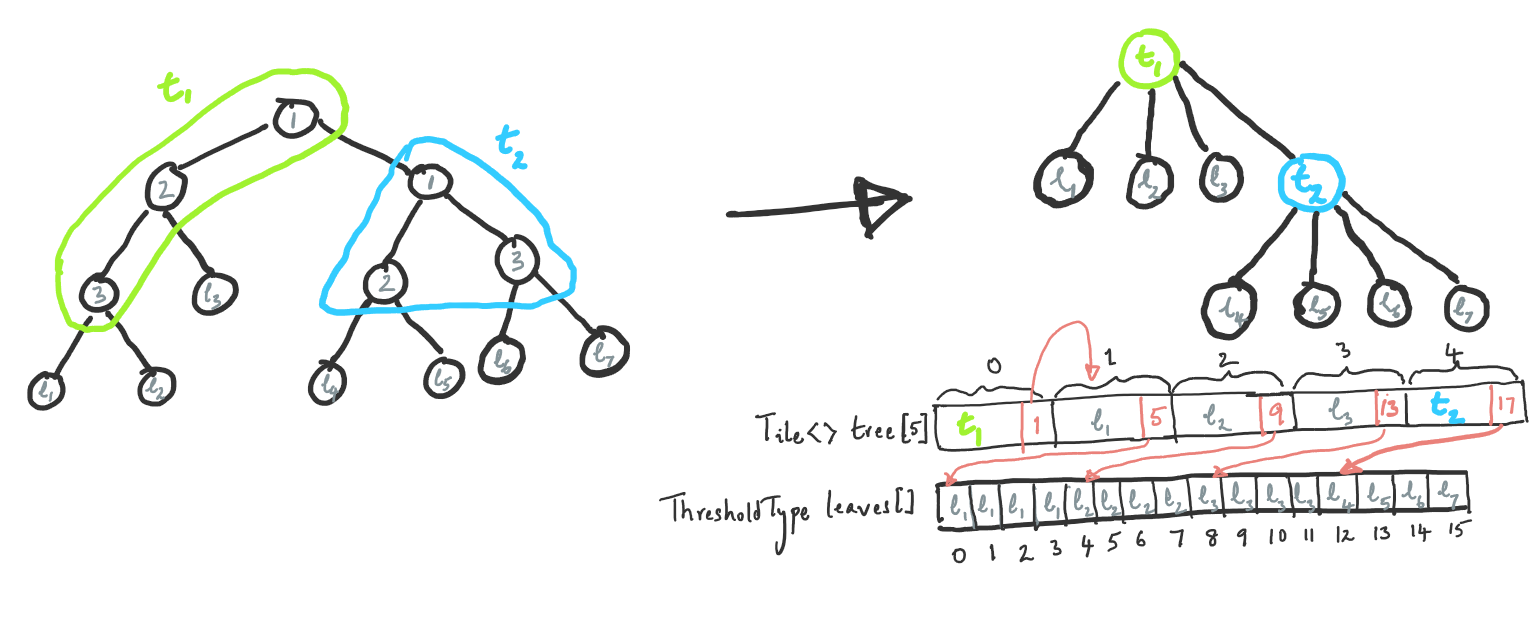
\includegraphics[width=\linewidth]{figures/SparseRep_TileSize3.PNG}
  \caption{Sparse representation with tile size $n_t=3$}
  \label{Fig:SparseRep}
\end{figure}

Figure \ref{Fig:SparseRep} shows some of the details of the sparse representation.
The tree on the left of the diagram is the actual decision tree with the nodes grouped into tiles $t_1$ and $t_2$. The tree on the right is the tree of tiles. The arrays depicted below show how the tree is represented in memory. The first array ($\texttt{tree}$) is an array of tiles and has 5 elements. Each element of the array represents a single tile and has the thresholds of the nodes, the feature indices, a tile shape ID and a pointer to the first child (shown explicitly in red). 

As a specific example, consider the tile $t_1$. The tile has four children -- $l_1$, $l_2$, $l_3$ and $t_2$ in that order (left to right). These tiles are stored contiguously in the $\texttt{tree}$ array and a pointer to the first of these, $l_1$ is stored in the tile $t_1$ (the index 1 is stored in the tile $t_1$ as shown). 

Now consider the tile $t_2$. Since all children of the tile $t_2$ are leaves, they are all moved into the $\texttt{leaves}$ array. To store a pointer into the $\texttt{leaves}$ array, we add $\texttt{len(tree)}$ to the element index in the $\texttt{leaves}$ array. The tile $t_2$'s child is the element at index 12 of the $\texttt{leaves}$ array. Therefore, the index $12 + 5 = 17$ is stored in the tile $t_2$. (Any index $i$ that is greater than the length of the $\texttt{tree}$ array is regarded as an index into the $\texttt{leaves}$ array. The index into the $\texttt{leaves}$ array is $i - \texttt{len(tree)}$.)

The other aspect of the representation is that an extra hop is added for the leaves $l_1$, $l_2$ and $l_3$ in order to simplify code generation. This enforces the invariant that all leaves are stored in the leaves array and  simplifies checking whether we've reached a leaf. Therefore, 4 new leaves are added as children for each of the original leaves $l_1$, $l_2$ and $l_3$. Each of these 12 newly added leaves has the same value as its parent. These are the first 12 elements of the $\texttt{leaves}$ array.

Even though we currently have implementations of the two representations detailed in sections \ref{sec:ArrayBased} and \ref{sec:SparseRep}, support for other representations is not hard to add. All optimizing passes that work on the high level and mid level IR will continue to work as is. Programmers need only provide new lowering passes for a few operations in the low level IR.

\subsection{Tree ordering}
\label{sec:treeorder}
Specializing the code for each tree in a model comes at a cost. First the code generator needs to generate different code for different trees potentially increasing the size of the generated code. Second some cross tree optimizations (applied at the lower levels of abstraction) like tree walk interleaving require that the multiple trees share identical code. In order to handle
this, \Treebeard{} pads trees with dummy nodes to make them balanced and then sorts the trees by their depth, so that trees of same depth can share code. Padding is only done for almost balanced trees (as generated by basic tiling), this is ensured by only adding up to a fixed fraction of dummy nodes.  
\TODO{Kr : Can we say something better above. If not can we add a threshold say 10\%?. Note : need to mention unrolling of padded sections in MIR.}
%This ensures that all trees with equal depth are grouped together.
 Once this is done, 
the loop over the trees is fissed so that each of the resulting loops only walks trees of a single depth. Consider for example a 
forest with 4 trees $T_1$, $T_2$, $T_3$, and $T_4$ in that order. Further, assume that $T_1$ and $T_4$ have depth 2 while $T_2$ and $T_3$
have depth 3. First, Treebeard reorders the trees to be in the order $T_1$, $T_4$, $T_2$, $T_3$. Then, the loop over the trees is fissed
as shown in the following listing.

% loop transformations for uniform tiling (splitting) 
\begin{lstlisting}{style=c++}
  forest = ensemble(...)
  for i = 0 to batchSize step 1 {
    prediction = 0
    for t = 0 to 2 step 1 {
      tree = getTree(forest, t) 
      node = getRoot(tree)
      node = traverseTreeTile(tree, node, rows[i])
      treePrediction = getLeafValue(tree, node)
      prediction = prediction + treePrediction
    }
    for t = 2 to 4 step 1 {
      tree = getTree(forest, t) 
      node = getRoot(tree)
      node = traverseTreeTile(tree, node, rows[i])
      node = traverseTreeTile(tree, node, rows[i])
      treePrediction = getLeafValue(tree, node)
      prediction = prediction + treePrediction
    }
    predictions[i] = prediction
  }  
\end{lstlisting}


\section{Loop optimizations at mid level}
\subsection{Tree Walk Interleaving}
A key bottleneck we found when we profiled code generated from tiled walks (even after vectorization) was that true dependencies between instructions were still causing
a significant number of processor stalls. Performing a walk with a single input-tree pair was not providing enough independent instructions to keep the processor busy. IN order to address this \Treebeard{} applies an unroll and jam transformation on the inner most loops of the loop nest. This has 
the effect of walking multiple tree and input row pairs in an interleaved fashion. 
This mitigates the dependency stalls by enabling scheduling of instructions from independent tree walks. 

This optimization is performed in two steps. 
First a pass on the mid-level IR transforms the loop structure. 
The following listing shows the mid-level IR when the inner loop over the input rows is unrolled 
by a factor of 2 and the two resulting tree walks are jammed together.

\begin{lstlisting}[style=c++]
  forest = ensemble(...)
  for t = 0 to numTrees step 1 {
    for i = 0 to batchSize step 2 {
      tree = getTree(forest, t)
      prediction1, prediction2 = InterleavedWalk((tree, rows[i]), (tree, rows[i+1]))
    }
  }
\end{lstlisting}
Next when lowering, the operations to traverse each of the tree, input row pairs 
(the arguments to the \texttt{InterleavedWalk}) are interleaved. One step of the interleaved 
walk is listed below. 
\begin{lstlisting}[style=c++]
  // ... 
  n1 = n2 = getRoot(tree)
  // ...
  threshold1 = loadThresholds(n1)
  threshold2 = loadThresholds(n2)
  featureIndex1 = loadFeatureIndices(n1)
  featureIndex2 = loadFeatureIndices(n2)
  feature1 = rows[i][featureIndex1]
  feature2 = rows[i][featureIndex2]
  pred1 = feature1 < threshold1
  pred2 = feature2 < threshold2
  n1 = getChildNode(n1, pred1)
  n2 = getChildNode(n2, pred2)
  // ...
\end{lstlisting}

\CommentOut{
These transformations are fairly general and are not aware of the in memory representation of the model. Therefore, they 
are reusable across different in memory representations - the ones that are currently built into Treebeard or ones that 
maybe added in the future.
\TODO{AP I feel the way this section is currently written makes the optimization seem extremely trivial. Is there a different 
way to present it?}
}
\subsection{Loop peeling and walk unrolling}
\Treebeard{} splits the loop that performs a tree walk into two parts. As can be made aware (through a simple pass on the IR) of the depth of the first leaf in a tree, it peels and introduces a \op{prologue} loop that walks down the tree a constant number of steps (up to first leaf) and then performs the rest of the tree walk in a separate loop. Next \Treebeard{} unrolls the prologue completely, avoiding all traversal induced branching in it.

Note that for trees where \Treebeard{} has already padded and balanced the tree (Section~\ref{sec:treeorder}), walk unrolling completely avoids all traversal induced spills.
\TODO{kr: Add example?}


\subsection{Parallelization}
Currently, \Treebeard{} performs a naive parallelization of the inference computation. When parallelism is enabled, the 
loop over the input rows is parallelized using a parallel for construct in MLIR. Treebeard rewrites 
the mid-level IR by tiling the loop over the input rows with a tile size equal to the number of cores. 
As a concrete example, consider the case where we intend to perform inference using a model with 4 trees 
on a batch of 64 rows. Further, assume that we wish to parallelize this computation across 8 cores. 
Treebeard then generates the following IR.
\begin{lstlisting}[style=c++]
  forest = ensemble(...)
  parallel.for i0 = 0 to 64 step 8 {
    for i1 = 0 to 8 step 1 {
      i = i0 + i1
      prediction = 0
      for t = 0 to 4 step 1 {
        tree = getTree(forest, t) 
        treePrediction = WalkTree(tree, rows[i])
        prediction = prediction + treePrediction
      }
      predictions[i] = prediction
    }
  }
\end{lstlisting}
Currently, \Treebeard{} does not perform other standard parallelization optimizations  (such as loop tiling) as they are generic and independent of the problem domain. We leave a more thorough exploration of parallelizing decision trees
to future work.

\section{Low level optimizations}
\subsection{Vectorization}
\label{sec:Vectorization}
Vectorization performed by Treebeard is enabled by the tiling transformations described in section \ref{sec:Tiling}. 
When the low level IR is translated to LLVM IR, Treebeard generates LLVM instructions that operate on the threholds and feature indices 
of nodes within a tile in a vector fashion. Therefore, thresholds and feature indices are loaded using vector loads and predicates are 
evaluated using vector comparisons. These vector LLVM IR instructions are then converted to vector instructions in the target ISA by 
the LLVM JIT.

The below listing shows some of the details of a vectorized tree walk. 
\begin{lstlisting}[style=c++]
  // A lookup table that determines the child index of
  // the next tile given the tile shape and the outcome
  // of the vector comparison on the current tile
  int16_t LUT[NUM_TILE_SHAPES, pow(2, TileSize)]
  
  ResultType Prediction_Function(...) {
    // ...
    Node n = getRoot(tree)
    while (isLeaf(tree, n)==false) do {
      thresholds = loadThresholds(tree, n)
      featureIndices = loadFeatureIndices(tree, n)
      // Gather required feature from the current row
      features = rows[i][featureIndices]
      // Vector comparison of features and thresholds
      comparison = features < thresholds
      
      // Pack bits in comparison vector into an integer
      comparisonIndex = combineBitsIntoInt(comparison)
      
      // Get child index of tile we need to move to
      tileShape = loadTileShape(tree, n)
      childIndex = LUT[tileShapeID, comparisonIndex]
      
      // Move to the correct child of the current node
      n = getChildNode(tree, n, childIndex) 
    }
    ThresholdType prediction = getLeafValue(n)
    // ...
  }  
\end{lstlisting}
To evaluate the current tile, the vector of thresholds is first loaded (\texttt{loadThresholds}). This vector contains the thresholds of all nodes in the tile. Then, the features required for comparison are gathered into a vector (lines 11 and 13). The feature vector is compared to the threshold vector and the child tile to move to is determined (lines 15 to 25). More details about tile shapes and the look up table are presented in subsequent sections.

\subsubsection{Tile Shapes}
Informally, the \textbf{\emph{tile shape}} is the shape of the region that encloses all nodes in a tile in a diagram of the decision tree. More formally, for a tile size $n_t$, each unique legal binary tree containing $n_t$ nodes (nodes being indistinguishable) corresponds to a tile shape.

Figure \ref{Fig:TileSize3Shapes} enumerates all tile shapes with a tile size of 3. There are a total of 5 tile shapes with size 3. The number of tile shapes with a tile size $n_t$, denoted by $NTS(n_t)$ is given by the following equation. 

\begin{equation}
  NTS(n) = \sum_{k=0}^{n-1} NTS(k) \times NTS(n-k-1)
\end{equation}

where $NTS(0) = NTS(1) = 1$.

\begin{figure}
  \centering
  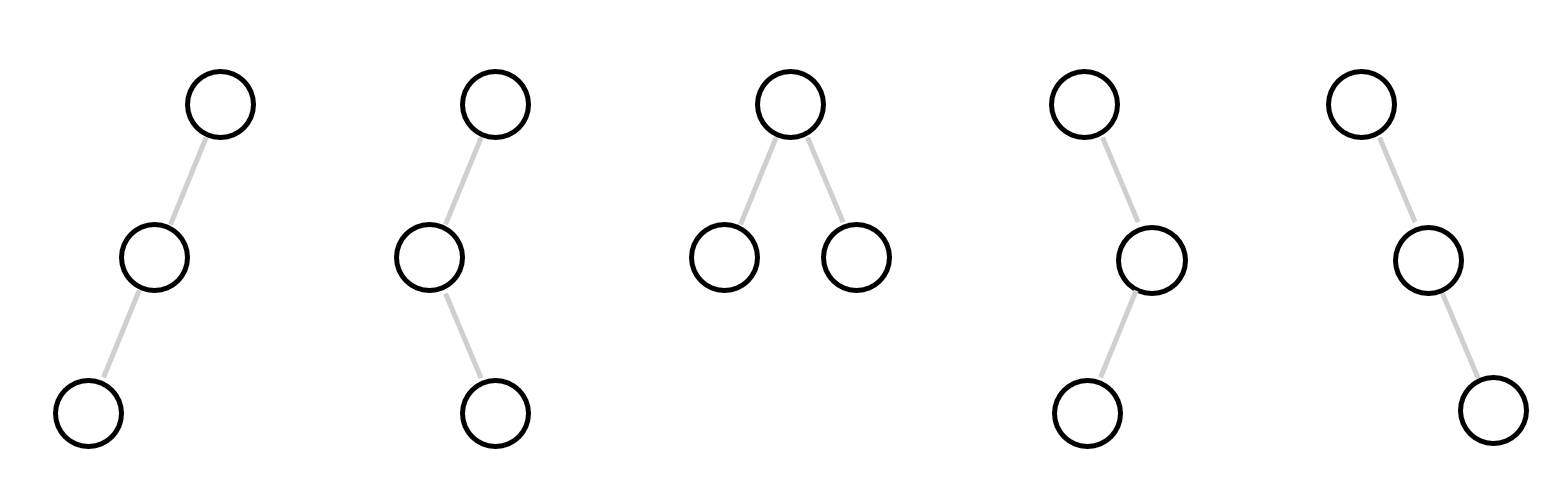
\includegraphics[width=\linewidth]{figures/TileShapes_Size3.PNG}
  \caption{All possible tile shapes with tile size $n_t=3$}
  \label{Fig:TileSize3Shapes}
\end{figure}

\subsubsection{Tile Shapes and Decision Tree Inference}
\label{Sec:TileShapesAndDecisionTreeInference}
Treebeard uses vector instructions to accelerate decision tree walks. Vector instructions are used to evaluate the predicates of all the nodes in a tile simultaneously. However, once the predicates of all the nodes in the tile are evaluated, computing the next tile to move to, given the outcome of the comparison depends on the tile shape of the current tile. To illustrate this problem, consider the case of the tiles of size 3 shown in figure \ref{Fig:TileTraversalTileSize3}. 
\begin{figure}
  \centering
  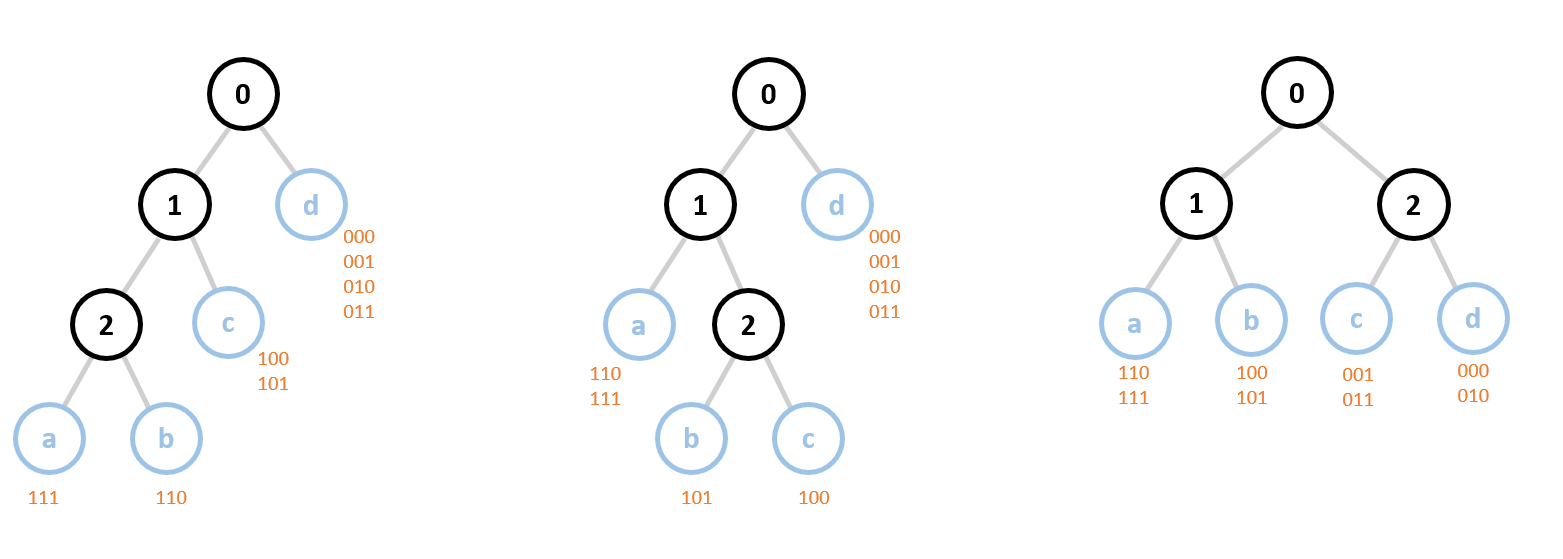
\includegraphics[width=\linewidth]{figures/TileTraversal_Size3.PNG}
  \caption{Example tile traversals with tile size $n_t=3$}
  \label{Fig:TileTraversalTileSize3}
\end{figure}
The diagram shows 3 of the 5 possible tile shapes for a tile size of 3. The nodes drawn in black are members of the tile $t_1$. The nodes in blue are the entry nodes of the children tiles of $t_1$. \TODO{Define entry nodes}

% To traverse a tile on an input row, first, the predicate of each node in the tile is computed. Subsequently, we need to determine which of the child tiles to move to next. Note that a true predicte (bit value 1) on a node implies a move to the left child and a false predicate (bit value 0) implies a move to the right child.

In the diagram, the bit strings (written in red) show which child we need to move to given the outcomes of the comparison. The bits represent the comparison outcomes of nodes and are in the order of the nodes in the tile -- marked 0, 1 and 2 in the diagram, i.e., the MSB is the predicate outcome of node 0 and the LSB the predicate outcome of node 2. For example, for the first tile shape, if the predicates of all nodes are true (i.e. the comparison outcome is 111), the next node to evaluate is $a$. 
% However, if the predicate of node 1 is false, then we need to move to $d$ regardless of the outcomes of nodes 2 and 3.
It is easy to see from the diagram that, depending on the tile shape, the same predicate outcomes can mean moving to different children. For example, for the outcome "011", the next tile is the 4th child (node $d$) for the first two tile shapes while it is the 3rd child for the other tile shape (node $c$).

\subsubsection{Lookup Table}
\label{sec:LookupTable}
A lookup table (LUT) is used to solve the problem described in section \ref{Sec:TileShapesAndDecisionTreeInference}, i.e. given the outcome of the comparisons of all nodes in a tile, determine the child tile we should evaluate next. The LUT is indexed by the tile shape and the comparison outcome. Formally, the LUT is a map.
\[
LUT : (TileShape, < Boolean \times n_t >) \rightarrow [0, n_t] \subset \mathbb{N}
\]

where $n_t$ is the tile size, $< Boolean \times n_t >$ is a vector of $n_t$ booleans. The value returned by the LUT is the index of the child of the current tile that should be evaluated next. For example, if we are evaluating the first tile $t$ in figure \ref{Fig:TileTraversalTileSize3}, and the result of the comparison is 110, then $LUT(TileShape(t), 110)=1$ since the tile we need to evaluate next is the tile with node $b$, which is the second child of the current tile.

In order to realize this LUT in generated code, Treebeard associates a non-negative integer ID with every unique tile shape of the given tile size. The result of the comparison, a vector of booleans, can be interpreted as a 64-bit integer. Therefore, the LUT can be implemented as a 2 dimensional array.
% \begin{lstlisting}{style=c++}
%   int16_t LUT[NTS(n_t), pow(2, n_t)]  
% \end{lstlisting}
Treebeard computes the values in the LUT statically as the tile size is a compile time constant.
\TODO{AP What comes after subsubsection?}

\subsection{In Memory Representation of Tiled Trees}
Treebeard currently has two in memory representations for tiled trees - an array based representation and a sparse representation. Both representations use an array of structs to represent all tiles of the model. 

\subsubsection{Array Based Representation}
\label{sec:ArrayBased}
Each tree in the model is represented as an array of tiles using the standard representation of trees as arrays. The root node is at index 0 and for a node at index $n$ in the array, the index of its $i^{th}$ child is given by $(n_t + 1) n + (i + 1)$ (nodes in the tree of tiles have $n_t + 1$ children). A tile is represented by an object of the following struct.
\begin{lstlisting}{style=c++}
  struct Tile {
    // A vector of TileSize elements
    <ThresholdType x TileSize> thresholds; 
    <FeatureIndexType x TileSize> featureIndices;
    // Integer that identifies the tile shape
    TileShapeIDType tileShapeID; 
  };  
\end{lstlisting}
\TODO{AP Is this level of detail really needed? Also, the vector type notation needs to be introduced somewhere.}
Even though this representation is simple and efficient for small models, the memory required for bigger models is very large. 
%The memory footprint is up to 20X that of the scalar representation.
This memory bloat causes performance problems because the span of the L1 TLB is not sufficient to efficiently translate 
addresses for the whole model. Storing leaves as full tiles (even though leaves just have to represent one value) and the
empty space introduced due to the array based representation of trees that are not complete account for most
of the increase.
%The sparse representation described next tries to address these issues. 

\subsubsection{Sparse Representation}
\label{sec:SparseRep}
The sparse representation tries to address the large memory footprint of the array based representation by doing the following.

\begin{itemize}
  \item We add a child pointer to each tile to eliminate the wasted space in the array representation. This points to the first child of the tile. All children of a tile are stored contiguously.
  \item Leaves are stored as a separate array of scalar values. Across all our benchmarks, after tiling a large fraction of 
  leaves are such that all their siblings are also leaves. Such leaves are directly moved into the leaves array. For leaves
  for which this property does not hold, an extra ``hop'' is added by making the original leaf tile a normal tile. All its
  children are made leaves with the same value as the original leaf.
\end{itemize}

\begin{figure}
  \centering
  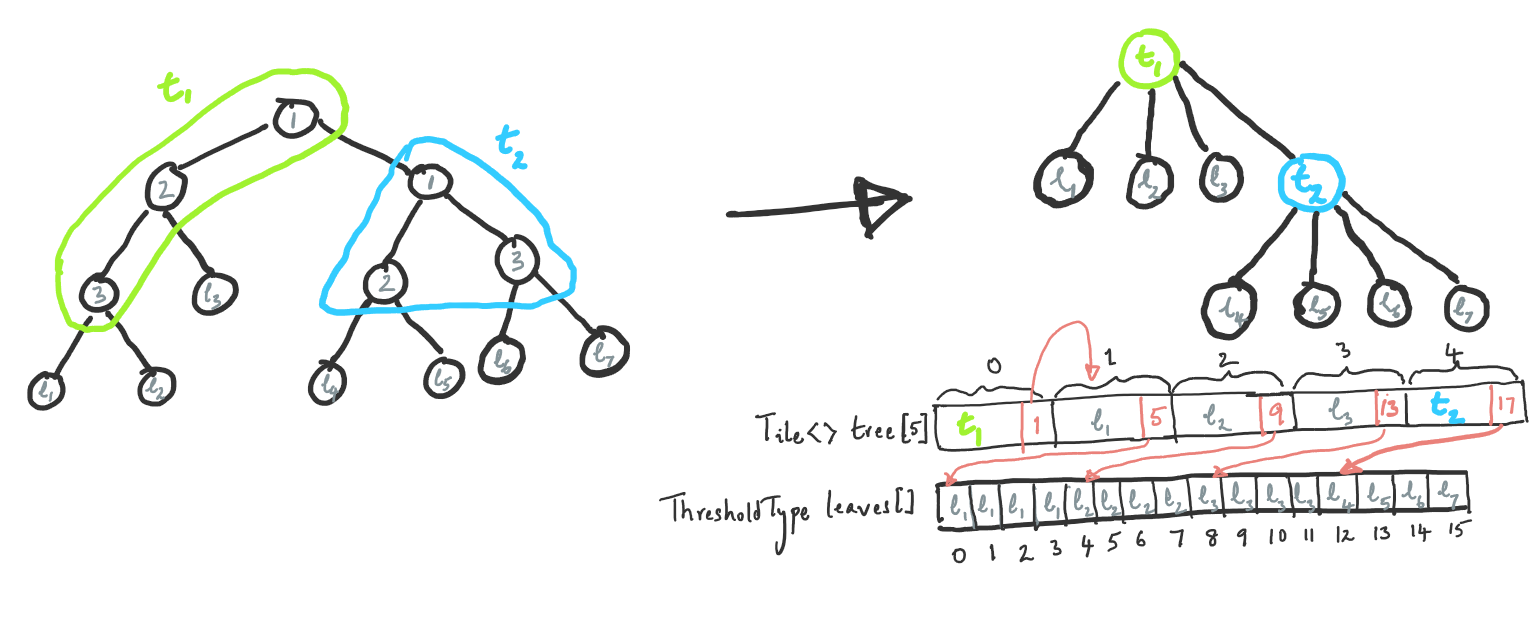
\includegraphics[width=\linewidth]{figures/SparseRep_TileSize3.PNG}
  \caption{Sparse representation with tile size $n_t=3$}
  \label{Fig:SparseRep}
\end{figure}

Figure \ref{Fig:SparseRep} shows some of the details of the sparse representation.
% The tree on the left of the diagram is the actual decision tree with the nodes grouped into tiles $t_1$ and $t_2$. The tree on the right is the tree of tiles.
The arrays depicted below show how the tree is represented in memory. The first array ($\texttt{tree}$) is an array of tiles 
and has 5 elements. Each element of the array represents a single tile and has the thresholds of the nodes, the feature
indices, a tile shape ID and a pointer to the first child (shown explicitly in red). 

As a specific example, consider the tile $t_1$. The tile has four children -- $l_1$, $l_2$, $l_3$ and $t_2$ in that order (left to right). These tiles are stored contiguously in the $\texttt{tree}$ array and a pointer to the first of these, $l_1$ is stored in the tile $t_1$ (the index 1 is stored in the tile $t_1$ as shown). 

Now consider the tile $t_2$. Since all children of the tile $t_2$ are leaves, they are all moved into the $\texttt{leaves}$ array.
To store a pointer into the $\texttt{leaves}$ array, we add $\texttt{len(tree)}$ to the element index in the $\texttt{leaves}$ array.
The tile $t_2$'s child is the element at index 12 of the $\texttt{leaves}$ array. Therefore, the index $12 + 5 = 17$ is stored in 
the tile $t_2$. Any index $i$ that is greater than the length of the $\texttt{tree}$ array is regarded as an index into the
$\texttt{leaves}$ array. The index into the $\texttt{leaves}$ array is $i - \texttt{len(tree)}$.

The other aspect of the representation is that an extra hop is added for the leaves $l_1$, $l_2$ and $l_3$ in order to simplify
code generation. This enforces the invariant that all leaves are stored in the leaves array and  simplifies checking whether
we've reached a leaf. Therefore, 4 new leaves are added as children for each of the original leaves $l_1$, $l_2$ and $l_3$. 
Each of these 12 newly added leaves has the same value as its parent. These are the first 12 elements of the $\texttt{leaves}$ array.

Even though we currently have implementations of the two representations detailed in sections \ref{sec:ArrayBased} 
and \ref{sec:SparseRep}, support for other representations is not hard to add. All optimizing passes that work on 
the high level and mid level IR will continue to work as is. Programmers need only provide new lowering passes for
a few operations in the low level IR.

\subsubsection{Code Generation for Probability Based Tiling}
As probability based tiling pulls the most probable leaves of a decision tree nearest the root, it poses 
some implementation challenges. By design, the tiling process makes the tree of tiles 
imbalanced. The array based representation (section \ref{sec:ArrayBased})
cannot be used because of the memory footprint increase (a large part of the tree is empty, but would need to be allocated).
On the other hand, the sparse representation in section \ref{sec:SparseRep} adds 
an extra hop for leaves that have non-leaf siblings. But this would mean that we add extra hops for 
the most probable leaves after probability based tiling which defeats the optimization.

We address these challenges using a code generation strategy. Treebeard peels 
the tree walk and specializes the leaf checks at higher levels to avoid the extra hop. Currently, 
we determine the maximum depth of leaves needed to cover 90 percent of the inputs and peel the tree 
walk by as many iterations. For example, consider the case where leaves until depth 2 are needed to 
cover 90 percent of the training input. Then, Treebeard generates the following IR. 

\begin{lstlisting}{style=c++}
    // ...
    tree = getTree(forest, t)
    node = getRoot(tree)
    node = traverseTreeTile(tree, node, rows[i])
    if (isLeafTile(node)) {
        treePrediction = getLeafValue(tree, node)
    } else {    
        node = traverseTreeTile(tree, node, rows[i])
        if (isLeafTile(node)) {
            treePrediction = getLeafValue(tree, node)
        } else {    
            // Loop based traversal 
        }
    }
    treePrediction = getLeafValue(tree, node)
    // ...
\end{lstlisting}

The if statements check whether a node is a leaf tile and hence avoid the extra hop. 
%The memory 
%requirement is also not increased because only a small fraction of leaves are represented as full tiles.
While walk peeling is used to improve the performance of probability based tiling by specializing leaf tests,
the transformation is by itself general and can be used in different contexts. For example, it could be used 
to elide leaf checks until a depth $d$ is reached if we know all leaves are at a depth greater than $d$. 

One other issue that the code generator needs to handle is that walks of different trees in the same ensemble may 
need to be peeled to different depths. A strategy similar to what is used for uniform tiling is used to handle this.
Trees are reordered so that all trees 
with equal peeling depth are grouped together and the loops in the IR are fissed so that tree walks 
for these groups of trees can be specialized differently.
% This is very similar to the code generation strategy used for uniform tiling.


\section{Related Work}

\emph{Decision Tree Ensemble Compilers:}
Treelite\cite{Treelite} only supports generation of if-else style code and is not extensible.
Hummingbird\cite{Hummingbird} tries to compile decision tree models to tensor primitives so 
they can be integrated into tensor based frameworks like TensorFlow \cite{TensorFlow}.

\emph{Libraries:} Currently, the most popular systems for decision tree based models 
are libraries. XGBoost\cite{XGBoost} and LightGBM\cite{LightGBM} are the most  
popular gradient boosting libraries while scikit-learn\cite{Sklearn} is 
extremely popular for random forest models. These libraries implement both 
training and inference. 

\emph{Other Systems and Techniques}: 
Ren et al \cite{PortableVM} build an intermediate language and VM to 
enable SIMD execution of decision tree inference. The SIMD execution itself is implemented 
by hand in the VM and the VM needs to be reimplemented for every supported target architecture.
Additionally, even though they perform layout optimizations, their system doesn't perform 
any model specific optimizations. 

Tahoe, Vpred, CacheConscious1, QuickScorer, QuickScorer1, MilindTreeVectorization
Bliss?

Decision tree training parallelization references

%%%%%%% -- PAPER CONTENT ENDS -- %%%%%%%%


%%%%%%%%% -- BIB STYLE AND FILE -- %%%%%%%%
\bibliographystyle{IEEEtranS}
\bibliography{refs}
%%%%%%%%%%%%%%%%%%%%%%%%%%%%%%%%%%%%

\end{document}
